
\documentclass[12pt]{report}

\usepackage{fullpage}
\usepackage{graphicx}
\usepackage{listings}
\usepackage{verbatim}
\usepackage{amsmath}
\usepackage{color}
\usepackage{hyperref}
 
\definecolor{codegreen}{rgb}{0,0.6,0}
\definecolor{codegray}{rgb}{0.5,0.5,0.5}
\definecolor{codepurple}{rgb}{0.58,0,0.82}
\definecolor{backcolour}{rgb}{0.95,0.95,0.92}
 
\lstdefinestyle{mystyle}{
    backgroundcolor=\color{backcolour},   
    commentstyle=\color{codegreen},
    keywordstyle=\color{magenta},
    numberstyle=\tiny\color{codegray},
    stringstyle=\color{codepurple},
    basicstyle=\footnotesize,
    breakatwhitespace=false,         
    breaklines=true,                 
    captionpos=b,                    
    keepspaces=true,                 
    numbers=left,                    
    numbersep=5pt,                  
    showspaces=false,                
    showstringspaces=false,
    showtabs=false,                  
    tabsize=2
}
 
\lstset{style=mystyle}
\renewcommand{\baselinestretch}{2}
\author{Mohammed Nauman Sididque}
\title{Assignment 3 \\Information Retrieval \\ CS 834 \\ Fall 2017 }

\begin{document}
\maketitle
\tableofcontents
\chapter{Problem 6.2}
\section{Problem Statement}
Create a simple spelling corrector based on the noisy channel model. Use a single-word language model, and an error model where all errors with the same edit distance have the same probability. Only consider edit distances of 1 or 2. Implement your own edit distance calculator (example code can easily be found on the Web).
\section{Solution}
\subsection{Noisy Channel Model}
This problem has been solved using Wiki small dataset provided by the text book. Initially we need to find the words in the corpus. The corpus contains 3902115 words of which 225744 are unique. The output of the total words  is in file ``word\_list.txt'' which has been added to the Assignment3 folder of Github.\\
Code parsing out words from the wiki small dataset
\lstinputlisting[language=Python]{Problem6_2/WordList.py}
The next step was to find the unique words of from the list of total words. I used unix commands  as mentioned below:
\begin{lstlisting}[language=bash]
  $  sort word_list.txt | uniq -c > word_list_unique.txt 
\end{lstlisting}
This command sorts my word\_list file and counts all the unique words to save it to the file word\_list\_unique.txt
\begin{lstlisting}[language=bash]
  $   awk '{print $1}' word\_list_unique.txt > word_list_unique_frequency.txt 
\end{lstlisting}
This command cuts the frequency of unique words from word\_list\_unique.txt and saves to word\_list\_unique\_frequency.txt
\begin{lstlisting}[language=bash]
  $   awk '{print $2}' word_list_unique.txt > word_list_unique_.txt
\end{lstlisting}
This command cuts the unique words listed from word\_list\_unique.txt and saves to word\_list\_unique\_.txt
The above two files were then used by the code to save them to lists.
\lstinputlisting[language=Python]{Problem6_2/WordFrequency.py}
In caculating edit distance between strings insetion, deletion and replace have been considered. Transformation has not been implemented. \\
Code for calculating edit distance between two strings.
\lstinputlisting[language=Python]{Problem6_2/EditDistance.py}
Code for NoisyChannel Model
\lstinputlisting[language=Python]{Problem6_2/NoisyModel.py}
Noisy Channel Code
\[W = argmax_{w \epsilon V} P(x|w)P(w)\]
where W is  predicted word\\
$P(x|w)$ is the error model \\
P(w) is the document mode \\
The above equation states that the word which has the highest product of document model and  error model is the predicted word in noisy model channel. \\
\subsection{Steps for generating the predicted correct word using Noisy Channel Model}
\begin{description}
\item[$\bullet$] Parse out all posibble words from the corpus.
\item[$\bullet$] Identify all the unique words with their frequency from the word list. 
\item[$\bullet$] Calculate the edit distance of the input word with each unique word present in the word list of the corpus.
\item[$\bullet$]For each unique word in the corpus compute the probability product using equation 1 . 
\item[$\bullet$] Find the word with highest probability and that is your predicted correct word from corpus for the word entered by the user.   
\end{description}
\subsection{Assumptions}
\begin{description}
\item[$\ast$]Consider only those unique words which have an edit distance of 0, 1 or 2.
\item[$\ast$]Calculate the edit distnace if the first character of the unique word from corpus and word entered by user match.
\item[$\ast$]Calculate edit distance if the difference of the length if word entered by user and unique word from corpus is 1.
\item[$\ast$]The probability of error model have been provided with constant values. For edit distance 1 , the error model probability is set to 0.6 and for edit distance 2, the error model probability is set to 0.2.
\end{description}
\subsection{Outputs}
\begin{figure}[ht]
  \centering
  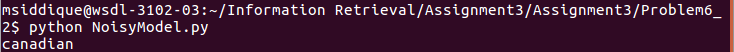
\includegraphics[width=1\textwidth]{Problem6_2/Screenshots/canadai.PNG}
  \caption{Output for input:canadai }
  \label{fig:1}
\end{figure}
\begin{figure}[ht]
  \centering
  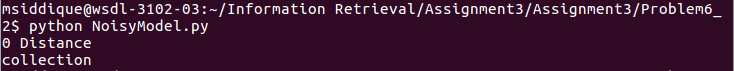
\includegraphics[width=1\textwidth]{Problem6_2/Screenshots/collection.PNG}
  \caption{Output for input:collection }
  \label{fig:1}
\end{figure}
\begin{figure}[ht]
  \centering
  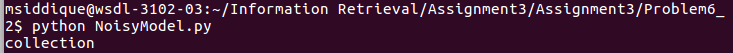
\includegraphics[width=1\textwidth]{Problem6_2/Screenshots/collectionz.PNG}
  \caption{Output for input:collectionz }
  \label{fig:1}
\end{figure}
\begin{figure}[ht]
  \centering
  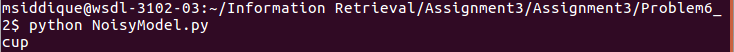
\includegraphics[width=1\textwidth]{Problem6_2/Screenshots/copr.PNG}
  \caption{Output for input:copr }
  \label{fig:1}
\end{figure}
\begin{figure}[ht]
  \centering
  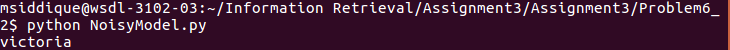
\includegraphics[width=1\textwidth]{Problem6_2/Screenshots/victora.PNG}
  \caption{Output for input:victora }
  \label{fig:1}
\end{figure}

\chapter{Problem 6.4}
\section{Problem Statement}
Assuming you had a gazetteer of place names available, sketch out an algorithm for detecting place names or locations in queries. Show examples of the types of queries where your algorithm would succeed and where it would fail.
\section{Solution}
\subsection{Assumption about the Location Gazetteer}
It does not accept any argument other than strings. It can not translate latitude and longitude, zipcodes and other aspects of address which rely on numerical value for translating address or location. 
\subsection{Description of the Algorithm}
It parses the query term and splits them to query terms on the basis of space, colon and other punctuation marks used frequently in the address. Intially the algorithm sends all the query terms to the location gazatter and if it is a hit it processes the query. In case of miss, it extracts each query term and sends them individually to the location gazatteer. In case of a hit, the index of the query term is saved and then the query term is split in two blocks with index term as mid point. For example, a sample query is Sushi in Norfolk Found. Each query term is passed individually to th location gazatteer. In case of Norfolk it is a hit. Now the query is split as Sushi in as first block , Found as second block and Norfolk is kept as index variable. The first half of the query terms are evaluated in reverse order starting from index location to zero position query term. Each time a query is formed by concatenating with the previous query term and send it to location gazatteer. In case of hit, the query tasks are perfomed but in case of a miss, the process is repeated again the previous query term is added to the query and checked with location gazatteer. This continues till all the elements prior to the index term have not been part of the query and been checked in the location gazatteer. If it is a overall miss, this step is then performed for query terms index to the end of the query terms. Each time a query term is appended to the query which has index query term to check for hit or miss with location gazatteer. If both the conditions fail then the index term is sent to location gazatteer and further actions are performed based on it. 
 
\verbatiminput{Problem6_4/Algorithm.txt}
Queries where it works:
\begin{description}
\item[$\bullet$]New York City
\item[$\bullet$]Royal Bazaar
\item[$\bullet$]Norfolk
\item[$\bullet$]Walmart Norfolk
\end{description}
Queries where it fails:
\begin{description}
\item[$\bullet$]IA 264
\item[$\bullet$]ZIP 23508
\item[$\bullet$]lat 88.0 long 12.34
\item[$\bullet$]ODU Address
\end{description}

\chapter{Problem 6.5}
\section{Problem Statement}
Describe the snippet generation algorithm in Galago. Would this algorithm work well for pages with little text content? Describe in detail how you would modify the algorithm to improve it.
\section{Solution}
\subsubsection{Dataset Used}
I am using wiki-small corpus downloaded from the book website to analyze the snippet generation algorithm in Galago.
\subsection{Description of Galago Snippet Algorithm} 
As shown in figure 3.1, Galago Search Engine presents search results with snippets for each indexed search result containing a title, URL and a short web summary to help the users find their desired result in quickly.
\begin{figure}[ht]
  \centering
  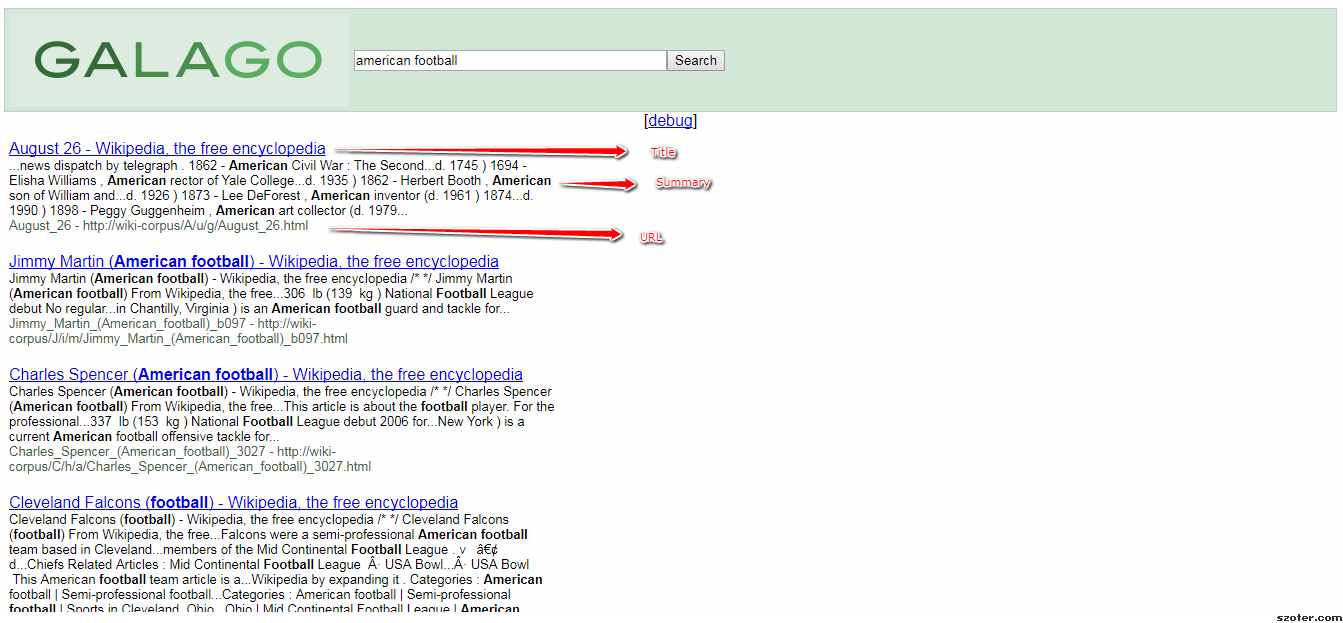
\includegraphics[width=1\textwidth]{Problem6_5/WebSnippet.PNG}
  \caption{Web Snippet In Galago}
  \label{fig:1}
\end{figure}

The title displayed in the snippets are extracted from header (h1, h2, h3....)  tags of the body of the webpage. The URLs displayed on search results have been modified to show standard URLs rather than the localhost extended URLs. The text for web summaries are extracted from the paragraph (p) tags of the body of the webpage. 
\begin{figure}[ht]
  \centering
  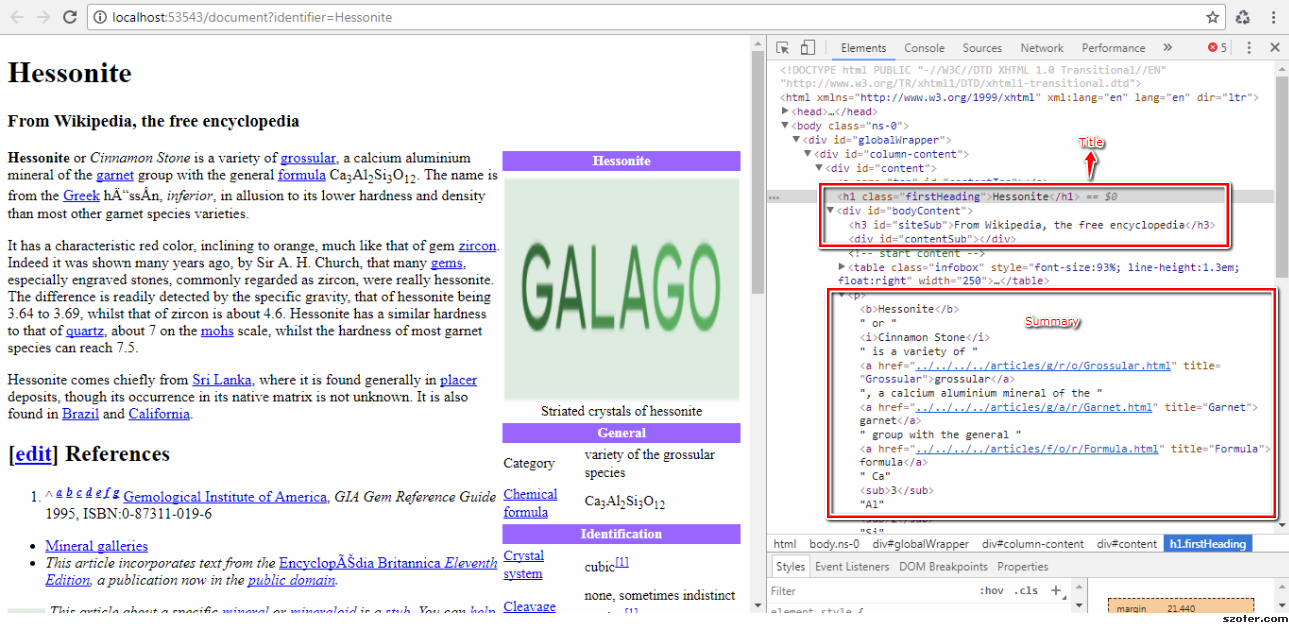
\includegraphics[width=1\textwidth]{Problem6_5/DescriptionofWebSnippets.PNG}
  \caption{Description of Web Snippet Generation}
  \label{fig:2}
\end{figure}

The text generated for web summaries are fragmented sentences rather than complete English language sentences. The texts extracted to form sentences for web summary contain the query terms in it. They do not stem the query terms for searching the word in the document. For query term gem stone, they search for the exact query terms and do not consider the words like gems or stones for forming web summaries. They roughly form fragmented sentences of ten words where the query term is the sixth term. In case, another query term falls within the range of fragmented sentence they extend the fragmented sentence by one. So, the general rule for the length of fragmented senteces is for each query term falling in the range of fragmented sentence the length increases by the number of query terms. For example, if three query terms lie in the fragmented sentence then the length will be tweleve as two extra words have been added for two extra query terms showing up in the fragmented sentence. When framing fragmented sentences they follow the order in the webpage.For example, if the webpage has three query terms and the web summary is of two fragmented sentence then, the fragmented sentences are constructed of the first two occurences of the query term. The length of the web summary in terms of fragmented sentences can be determined as roughly equal to half the query terms present in the webpage must occur in the web summary. For example, if a page contains fifteen query terms, then the web summary must contain seven to eight query terms in their web summary. But this approach could mean that the number of fragmented sentences could be in range of one to eight. 

\subsection{Little Text Content Problem}
   
One of the major problems with the Galago Snippet Generation algorithm with little text content is it might not produce any web summary if the query terms do not exactly match the words in the documents. As shown in figure 3.3, a web page with just a paragraph of text to validate our problem for little text content problem. For a search query gem stone the search result does not contain any web summary for this page as shown in figure 3.4. Although, the webpage does have one occurence of word gems which is a plural form of gem which can be seen in figure 3.3. So, with little text content it is very tricky for the Galago snippet generation algorithm to find the exact query terms each time in the document but without stemming of query terms it is bound to produce no web summary almost every time on my search request.   
\begin{figure}[ht]
  \centering
  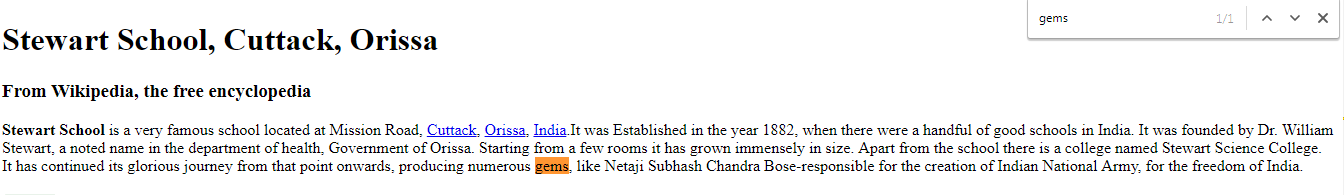
\includegraphics[width=1\textwidth]{Problem6_5/LittleTextContent.PNG}
  \caption{Document containing query term}
  \label{fig:3}
\end{figure}

\begin{figure}[ht]
  \centering
  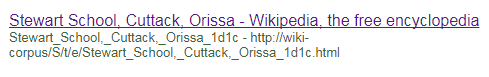
\includegraphics[width=1\textwidth]{Problem6_5/NoWebSummary.PNG}
  \caption{No Web summary generated for Query Term: Gem Stone}
  \label{fig:4}
\end{figure}

\subsection{Improvements to the Algorithm}

Firstly, the query terms need to be stemmed for incorporating their plural and other verb forms, which will help in generating web summaries for even little text content webpages.Secondly, the web summaries are supposed to be an abstract to the document, so the algorithm could extract some fragmented sentences from the metadata or the links which refer to the page rather than every time relying on the query term search in the socument. Thirdly, the length of web summaries needs to have some minimum and maximum threshold as it becomes a story when the search result contains five or greater sentences in web summary. The algorithm could even implement a feedback mechanism or analyze the clickthrough logs to underdstand the reasons for clickthrough inversions related to web summaries. The length of fragmented sentences do not need to be hard bound by any length but rather should convey meaningful information relating the the page.  
 
\chapter{Problem 6.9}
\section{Problem Statement}
Give five examples of web page translation that you think is poor. Why do you think the translation failed?
\section{Solution}
I chose to translate webpages from Hindi to English and from Urdu to English. This was done due to my familiarity with these languages which help me understand in detail the problems happening in translated version of the webpage.
\subsection{Aaj Tak Website}
It is a hindi news website. I loaded the webpage in the hindi and translated it to english by selection the option of translate to english on right click of the webpage. The reason for choosing this website as a bad translation is due to one news in particular. In figure 4.2, there is a news on the left side of the figure saying ``Hardline never reached Sibal's meeting''. The original news in hindi as shown in figure 4.1, says "The deadline on reservation ended by Patels, Hardik did not attend meeting with Sibal".   \\ 
 Hardline never reached Sibal's meeting - English Version\\
The deadline on reservation ended by Patels, Hardik did not attend meeting with Sibal - Hindi Version translated to English by me\\
If I look at both the news they seem very different to me because in english they converted Hardik to Hardline where Hardik is name of a person and hardline is something no where related to a name but it changes the whole narrative to the news now reading the headlines.  
\begin{figure}[ht]
  \centering
  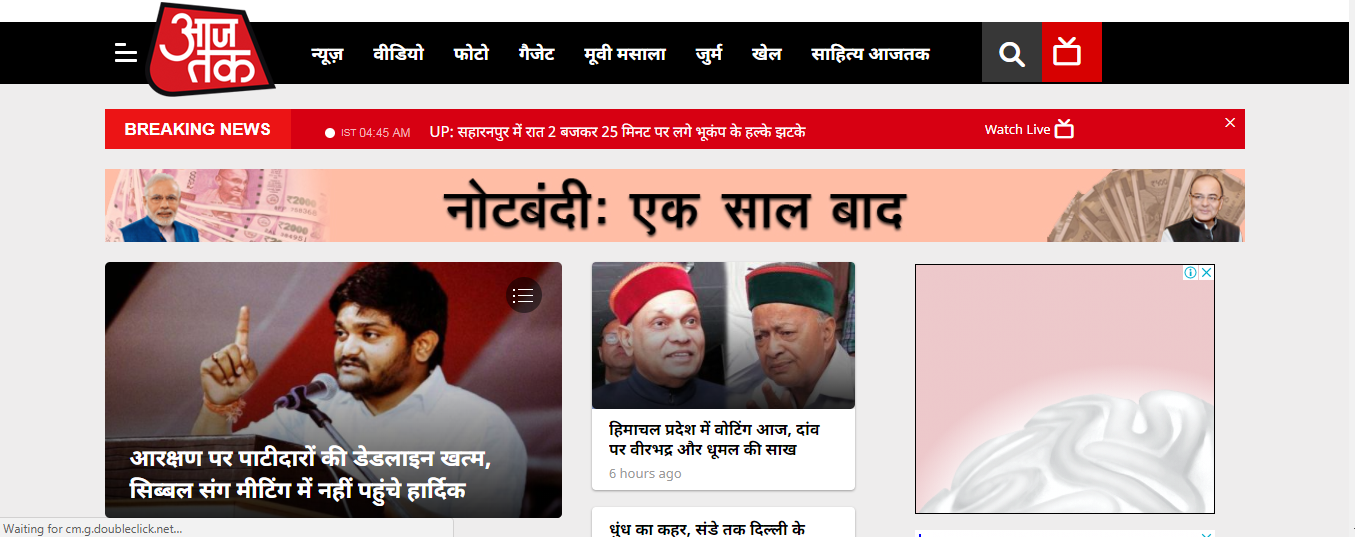
\includegraphics[width=1\textwidth]{Problem6_9/AajTak_Hindi.PNG}
  \caption{News website: Aaj Tak in Hindi}
  \label{fig:5}
\end{figure}

\begin{figure}[ht]
  \centering
  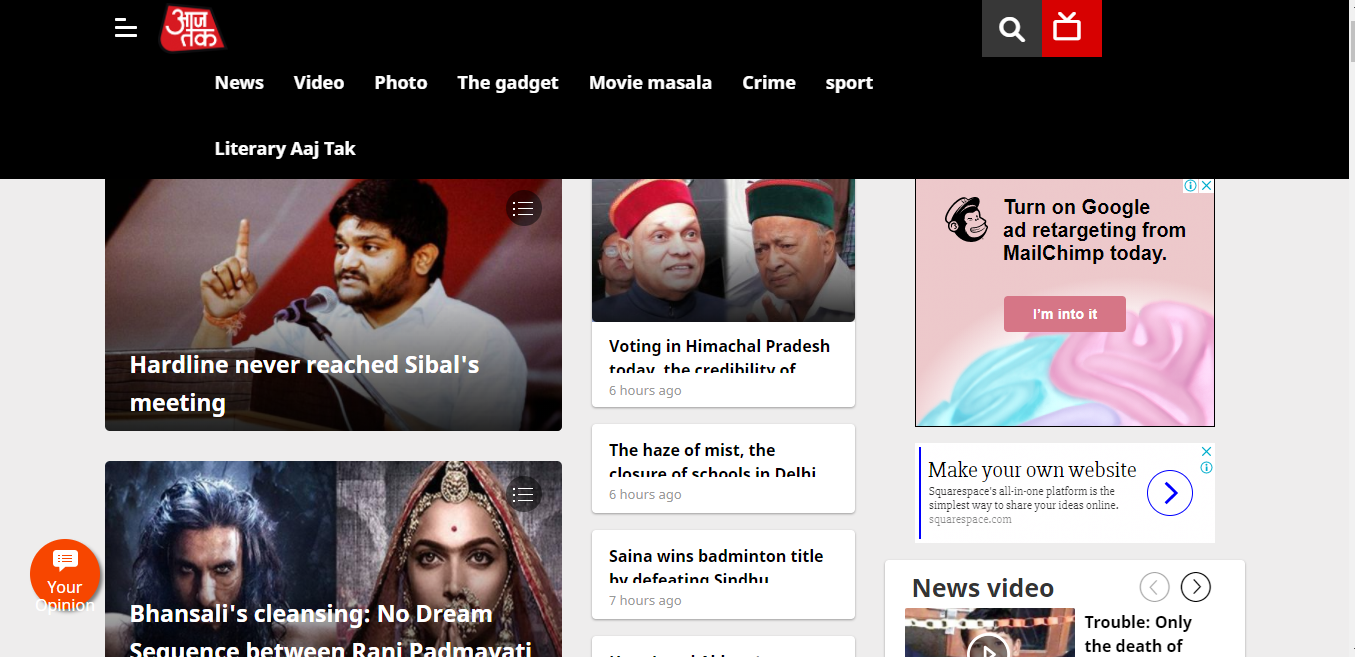
\includegraphics[width=1\textwidth]{Problem6_9/AajTak_English.PNG}
  \caption{News website: Aaj Tak in English}
  \label{fig:4}
\end{figure} 
\subsection{Aaj Tak News}
Figure 4.3 is an English translation of a news from Aaj Tak, a Hindi news daily. The paragraph shown in the figure is gramatically incorrect and looks like the news in Hindi has been literally converted to English leaving out the rules of English language grammer.
 \begin{figure}[ht]
  \centering
  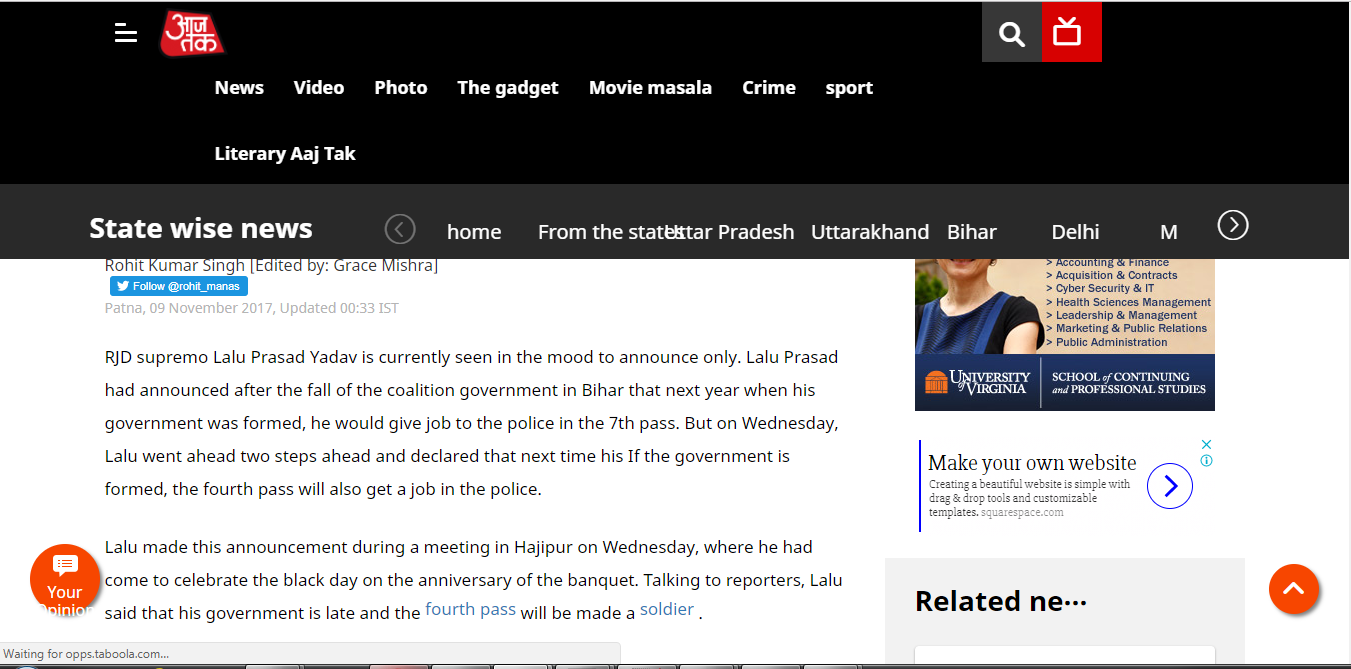
\includegraphics[width=1\textwidth]{Problem6_9/AajTak_News_English.PNG}
  \caption{News website: Aaj Tak News translated to English}
  \label{fig:6}
\end{figure}
\subsection{Dainik Bhaskar}
It is a Hindi news website. The paragraph of news translated in English as shown in figure 4.5 is not grammatically acceptable. There are numerous instances of wrong usage of capital and small letters and punctuations. 
\begin{figure}[ht]
  \centering
  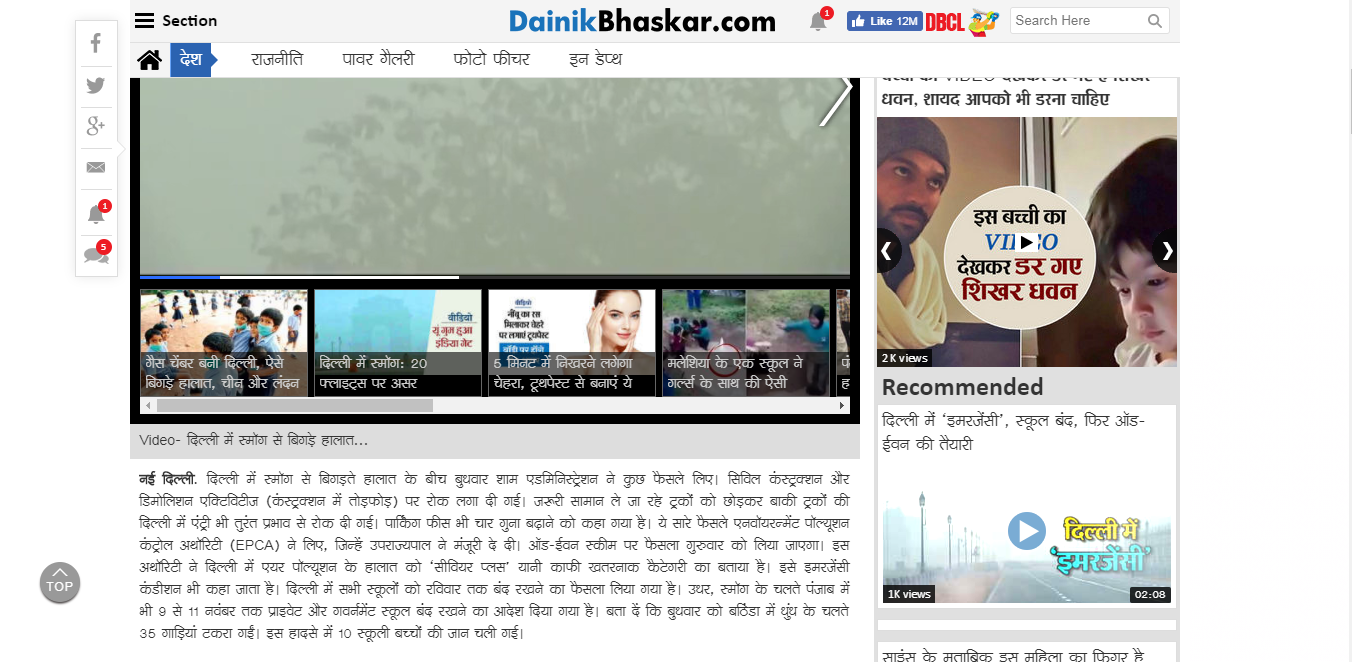
\includegraphics[width=1\textwidth]{Problem6_9/DainikBhaskar_Hindi.PNG}
  \caption{News website: Dainik Bhaskar in Hindi}
  \label{fig:6}
\end{figure}

\begin{figure}[ht]
  \centering
  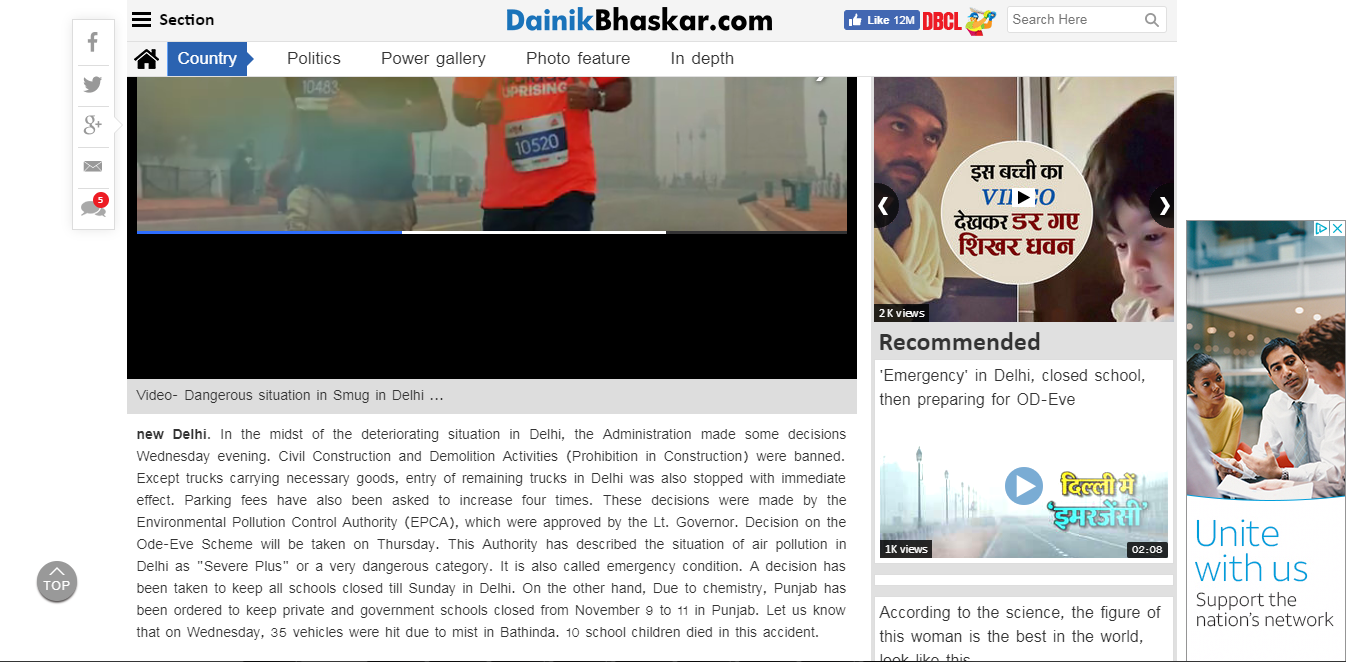
\includegraphics[width=1\textwidth]{Problem6_9/DainikBhaskar_English.PNG}
  \caption{News website: Dainik Bhaskar in English}
  \label{fig:7}
\end{figure} 
\subsection{Urdu Newspaper}
Figure 4.6 is an English translation of a news from Urdu newspaper. The texts in English are right to left aligned which is just a copy of the way urdu is written. Few proper nouns containing names of people mentioned in the news are wrong.
\begin{figure}[ht]
  \centering
  \includegraphics[width=1\textwidth]{Problem6_9/Urdu_newspaper_English.PNG}
  \caption{News website: Urdu Newspaper translated to English}
  \label{fig:7}
\end{figure} 
\subsection{Urdu Newspaper from Pakistan}
Figure 4.7 is an English translation of a news from Pakistani Urdu newspaper. The texts in English are right to left aligned which is just a copy of the way urdu is written. The most standout things to notice int he figure are the commas(,). They have been inverted in the document making the translated version look very rudimentary.
\begin{figure}[ht]
  \centering
  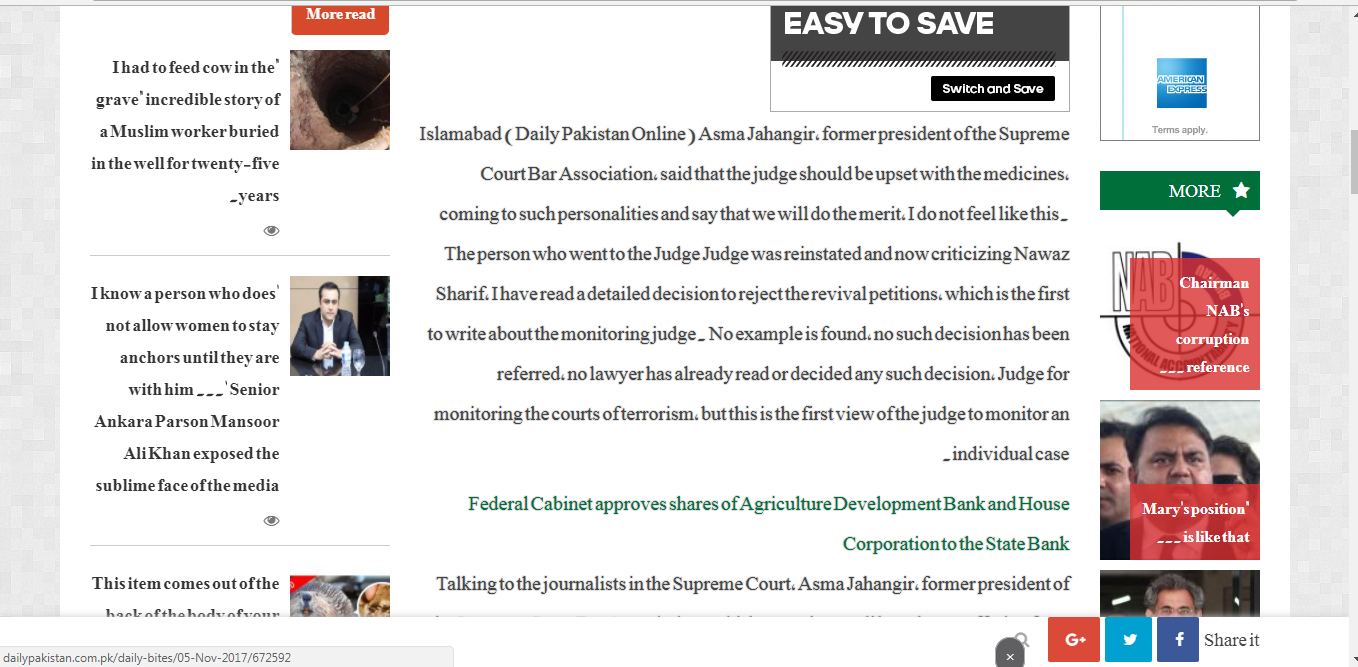
\includegraphics[width=1\textwidth]{Problem6_9/Urdu_newspaper_Pakistan.PNG}
  \caption{News website:Pakistani Urdu Newspaper translated to English}
  \label{fig:8}
\end{figure} 

\subsection{Possible reason for Wrong Translation}
 Firstly, a major flaw in the translation of a webpage to English was with proper nouns containing names of people which are unique to the geographical area. Google might not have those names in its dictionary and translated it incorrectly. Second, most standout flaw was translating from a language that has a right to left writing stlye to English. It did not have any understanding of the layout of the text. Thirdly, a number of punctuations appeared wierd in Urdu to English translation and it could be due to just reversing their direction and not keeping in to consideration that the writing style had been changed from right - left to left- right. Thirdly, one of the pages had a literal translation from Hindi to English. The reason could due to word to word text translation from Hindi to English. Machines lack the understanding to look at sentences and paragraphs in context and often translate them as they encounter on word by word or sentence by sentence. The reason for grammatically incorrect translation in English from Hindi could be due togeneral flow of English language which does not follow a strict rule and above all the machines translating it must be trained to form sentences out of ideas rather than words. The reason even we are having this conversation of improvement in translation is due to Google which does a fairly good job at translating webpages but it is difficult to train machines to understand the behaviour of natural languages which are influenced by people who use it rather than any harlined grammer.
\chapter{Problem 7.2}
\section{Problem Statement}
Can you think of another measure of similarity that could be used in the vector space model? Compare your measure with the cosine correlation using some example documents and queries with made-up weights. Browse the IR literature on the Web and see whether your measure has been studied (start with van Rijsbergen’s book).   
\section{Solution}
We can use Manhattan Distance to find similarity in vector space model.Manhattan distance is the distance between two points is the sum of the absolute differences of their Cartesian coordinates. The lesser the distance the closer they are or similar the two points are. We can use Manhattan Distance as the closer a value is to zero the more the document and query models.\\
Example:\\
In a plane with p1 at (x1, y1) and p2 at (x2, y2).\\
$ Manhattan Distance =  \lvert x1 - x2  \lvert  +  \lvert y1 - y2  \lvert $  \\
Suppose we have three documents D1,D2,D3 and three queries with q1,q2,q3.\\
The document vectors are assumed to be:\\
D1 = [0.8 ,0.7 ,0.6]\\
D2 = [1,0.5,0.3]\\
D3 = [0.7, 0.4, 0.9]\\
The query vectors are assumed to be:\\
q1 = [0.4, 0.2, 0.8]\\
q2 = [0.8, 0,3, 0.9]\\
q3 = [0.7, 0.9, 0.8 ]\\
Cosine Similarity\\
For Query q1 \\
D1 = $(0.8*0.4 )+ (0.7*0.2) + (0.6*0.8)/ \sqrt{(0.8^2 + 0.7^2 + 0.6^2) + (0.4^2 + 0.2^2 + 0.8^2)}$\\
D1 = $ (0.32 + 0.14 + 0.48)/1.59  = 0.59$\\
D2 = $(1*0.4 )+ (0.5*0.2) + (0.3*0.8)/ \sqrt{(1^2 + 0.5^2 + 0.3^2) + (0.4^2 + 0.2^2 + 0.8^2)}$\\
D2 = $ (0.4 + 0.1 + 0.24)/1.086  = 0.681$\\ 
D3 = $(0.7*0.4 )+ (0.4*0.2) + (0.9*0.8)/ \sqrt{(0.7^2 + 0.4^2 + 0.9^2) + (0.4^2 + 0.2^2 + 0.8^2)}$\\
D3 = $ (0.28 + 0.08 + 0.72)/1.517  = 0.712$\\ 
Manhattan Distance\\
For Query q1\\
D1 = $\lvert 0.8 - 0.4 \lvert + \lvert 0.7 - 0.2\lvert + \lvert 0.6- 0.8\lvert $\\
D1 = $ 0.4 + 0.5 + 0.2 = 1.1$\\ 
D2 = $\lvert 1 - 0.4 \lvert + \lvert 0.5 - 0.2\lvert + \lvert 0.3- 0.8\lvert $\\
D2 = $ 0.6 + 0.3 + 0.5 = 1.4$\\
D3 = $\lvert 0.7 - 0.4 \lvert + \lvert 0.4 - 0.2\lvert + \lvert 0.9- 0.8\lvert $\\
D3 = $ 0.3 + 0.2 + 0.1= 0.6$ \\


For query q1 the cosine similarity index for documents D1, D2 and D3 are 0.59, 0.681 and 0.712. The ranking of documents in respect to the query q1 is $D3 > D2 > D1$. For query q2 the Manhattan Distance for documents D1, D2 and D3 are 1.1, 1.4 and 0.6. The ranking of documents in respect to the query q1 is $D3 > D1> D2$.

Problems with Manhattan Distance
The major flaw in the Manhattan Distance is the non-normalized value. In the above example the distance could vary from 0 to 3 because there are three co-ordinates to each vector. So to normalize the values of Manhattan Distance we can divide it by the number of co-ordinates in each vector which results in Manhattan Distance in range of 0 to 1.

$Modified Manhattan Distance = (\lvert x1 - x2  \lvert  +  \lvert y1 - y2  \lvert)/ N $  \\
where N is the number of co-ordinates in each vector   

Cosine Similarity\\
For Query q2 \\
D1 = $(0.8*0.8 )+ (0.7*0.3) + (0.6*0.9)/ \sqrt{(0.8^2 + 0.7^2 + 0.6^2) + (0.8^2 + 0.3^2 + 0.9^2)}$\\
D1 = $ (0.64 + 0.21 + 0.54)/1.74  = 0.903$\\
D2 = $(1*0.8 )+ (0.5*0.3) + (0.3*0.9)/ \sqrt{(1^2 + 0.5^2 + 0.3^2) + (0.8^2 + 0.3^2 + 0.9^2)}$\\
D2 = $ (0.8 + 0.15 + 0.27)/1.697  = 0.719$\\ 
D3 = $(0.7*0.8 )+ (0.4*0.3) + (0.9*0.9)/ \sqrt{(0.7^2 + 0.4^2 + 0.9^2) + (0.8^2 + 0.3^2 + 0.9^2)}$\\
D3 = $ (0.56 + 0.12 + 0.81)/1.732  = 0.86$\\ 
Modified Manhattan Distance\\
For Query q2\\
D1 = $(\lvert 0.8 - 0.8 \lvert + \lvert 0.7 - 0.3\lvert + \lvert 0.6- 0.9\lvert) /3 $\\
D1 = $ (0 + 0.4 + 0.3)/3 = 0.234$\\ 
D2 = $(\lvert 1 - 0.8 \lvert + \lvert 0.5 - 0.3\lvert + \lvert 0.3- 0.9\lvert)/3 $\\
D2 = $( 0.2 + 0.2 + 0.6)/3 = 0.334$\\
D3 = $(\lvert 0.7 - 0.8 \lvert + \lvert 0.4 - 0.3\lvert + \lvert 0.9- 0.9\lvert)/3 $\\
D3 = $ (0.1 + 0.1 + 0)/3= 0.067$ \\

For query q1 the cosine similarity index for documents D1, D2 and D3 are 0.903, 0.719 and 0.86. The ranking of documents in respect to the query q1 is $D1 > D3 > D2$. For query q2 the Manhattan Distance for documents D1, D2 and D3 are 0.234, 0.334 and 0.067. The ranking of documents in respect to the query q1 is $D3 > D1> D2$.

Research Papers on calculating similarity using Manhattan Distance for Vector Space Model (used Google Scholar)\\
1. Evaluation of texture features for content-based image retrieval, by P Howarth, SM Rüger - CIVR, 2004 - Springer

There are a few other research papers related to Manhattan Distance for Vector Space Model but they are either a modified version of Manhattan Distance or they are talking about improvements over Manhattan Distance.

\chapter{Problem 7.7}
\section{Problem Statement}
What is the “bucket” analogy for a bigram language model? Give examples.   
\section{Solution}
In context of Information Retreival, Language Model is the ability to predict next word on the prior knowledge of the previous word. A language model for documents is the total vocabulary of the document which can be used to form query terms. A unigram language model is predicting the next word on the basis of their frerquency in the document. For example, if all the words present in the document are in a bucket and it is needed to contruct a new text with the bucket of words. A word is randomly chosen from the bucket without seeing in the bucket written down and the word is place back again in the bucket and then the search for next word happens in the similar fashion. It is the unigram language model where each word is independent of each other but are only just dependent on their occurence in the document. But, a bigram language model uses the prior knowledge of the previous word to predict the next word. The main advantage of bigram language model over unigram language model is that it considers the previous word in context to predict the next word unlike the unigram model which treats each word individually on their frequency. It can be shown by the below equation.

\[P_{bi}(t_1t_2t_3t_4) = P(t_1)P(t_2\vert t_1)P(t_3\vert t_2)P(t_4\vert t_3)\]

In respect to the bucket analogy, if all the words in the document are in a bucket and a new text is to be constructed using bigram language model,initially a word is picked from the bucket of words at random and writen down. Further on the bucket of words is replaced by the bucket of the words occuring with the prior word to select the next word and this process is continued where each time the bucket of words coming after the previous word is used to predict the next word.

For example, suppose there is a document that has following text.\\
i live in osaka .\\
i am a graduate student .\\
my school is in nara .\\

We want to find the probability of framing in osaka from the lanuage model using bigram model. It is defined by conditional probability of osaka occuring if in has already occured. The below equation says thatthe conditional probability of osaka with in is equal to the frequencies of occurence of  term in osaka divided by frequency of in.

\[P(osaka|in) = c(in osaka)/ c(in)\]
\[P(osaka|in) = 1/2 = 0.5\]

Similarly we want to predict the probability of nara occuring after in.

\[P(nara|in) = c(in nara)/ c(in)\]
\[P(nara|in) = 1/2 = 0.5\]

We want to predict school occuring after in.

\[P(school|in) = c(in school)/ c(in)\]
\[P(school|in) = 0/2 = 0\]

\chapter{Problem MLN1}
\section{Problem Statement}
using the small wikipedia example, choose 10 words and create stem classes as per the algorithm on pp. 191-192..   
\section{Solution}
\subsection{Description of Code}
The code uses a random list of words extracted from the word list generated by parsing out the wiki-small dataset. The code for parsing words from wiki-small dataset has been reused from problem 6.2 and is not part of the code for this problem. Porter The codde used Stemmer library of nltk package. The extacted words from the word list were stemmed to result in forming of 10 stems which will be used to build stem classes. The 10 stems, extarcted word list and the overall word list of the wiki-small dataset was passed as an argument createPorterStemmerClass() function which returns the stem classes by parsing out all of the word list and placing them in a stem class if it matches them. The stem classes are passed as an argument to the function countCooccurence() to return a 2-D matrix of co-occurence of stem words of each class in a window size of 50.     
\lstinputlisting[language=Python]{MLN1/StemClass.py}
\verbatiminput{MLN1/StemClass.txt}

\subsection{Results}
The first stem result is for stems class generated by parsing the word list of the wiki-small dataset. It does not account for co-occurence of the words in a stem class. The second output is empty, as none of the words in each stem class lied in a window size of 50,100 or 200. 

\chapter{Problem MLN2}
\section{Problem Statement}
Using the small wikipedia example, choose 10 words and compute MIM, EMIM, chi square, dice association measures for full document \& 5 word windows (cf. pp. 203-205).   
\section{Solution}
\subsection{Description of Code}
The code uses a random list of words extracted from the word list generated by parsing out the wiki-small dataset. The code for parsing words from wiki-small dataset has been reused from problem 6.2 and is not part of the code for this problem. I extracted the random words keeping an assumption that their frequencies must be greater than 100, so that I can get frequency values for the extracted words in a window size of five. I have provided constant values for the extracted word list, their frequencies and the totoal word list size of the wiki-small dataset. The extracted word list is passed as an argument to my function findWordOccurence() which creates a 10*10 matrix for storing frequency of two words occuring in a window size of five. The 2-D matrix of frequency, frequency of each extracted word list and total word count for wiki-small dataset have been used to calculate Dice Co-efficient, MIM, EMIM, Chi-square  for each pair of words in the extracted word list. The formulas for calculating each measure have been extracted from our text book.

\lstinputlisting[language=Python]{MLN2/WordOccurence.py}
\verbatiminput{MLN2/Result.txt}

\subsection{Results}

N = 3902115\\
word\_list =["canada","candidates","collections","competitive","composition","very", "couples","victoria", "weapon", "defence"]\\
word\_frequency\_list = [1090,106,105,104,104,1062,108,510,100,210] \\

The above three lines show the values that have been provided to the code based on my previous problem. First line contains N which represents the total number of words in the wiki-small dataset. Second line contains the extarcted word list and the last line has all the frequency values for each extarcted word list.The file for results shows values a 10*10 matrix which is the frequency of co-ocurrence of two query terms in a window size of 5. Further the file shows for every two query terms their values in different measure. The results queries have been shown only for queries which have non-zero values for each measure of query expansion. The list of frequent occuring query terms in a window size of 5 which can be used for query expansion are:\\
canada very \\
canada victoria\\
competitive very\\
very victoria\\
couples victoria\\
 
\end{document}